\section{Design pattern}
I \glossario{Design Pattern} descrivono la metodologia con cui affrontare problemi ricorrenti, fornendo degli standard che permettono di ottenere soluzioni eleganti e condivise.\\
La conoscenza dei Design Pattern favorisce la progettazione, il riuso e la manutenibilità del codice prodotto.\\
I principali Design Pattern vengono suddivisi in quattro categorie:
\begin{itemize}
	\item \textit{Architetturali}: affrontano il problema di progettazione di un sistema software fornendo uno schema di partenza su cui basare l'architettura (\glossario{MVC});
	\item \textit{Creazionali}: affrontano il problema di astrarre il sistema rendendolo indipendente dall'implementazione concreta delle sue componenti;
	\item \textit{Strutturali}: affrontano il problema riguardante la composizione delle classi e degli oggetti, sfruttando l'ereditarietà e l'aggregazione;
	\item \textit{Comportamentali}: affrontano il problema dell'interazione tra le componenti, definendo la funzione degli oggetti e il modo in cui interagiscono gli uni con gli altri.
\end{itemize}
Per una descrizione più approfondita e completa dei diversi Design Pattern utilizzati nella progettazione di \ProjectName{} si rimanda all'\appendice{app:design_pattern}. Di seguito viene invece descritto come sono stati utilizzati i diversi Design Pattern nella progettazione delle varie parti dell'architettura.

\subsection{Design Pattern Architetturali}

\subsubsection{MVC - Model View Controller}
\textbf{Scopo:}\\ 
Permette di separare le responsabilità dei diversi componenti dell'applicazione dividendo presentazione, controllo e operazioni sui dati. Questo rende il codice manutenibile e di più semplice interpretazione.\\
\textbf{Utilizzo:}\\
Viene utilizzato per affidare la gestione dell'interfaccia alla view, lasciando al model e al controller la gestione logica dell'applicazione, ed in particolare lo storage dei dati, l'interazione tra gli utenti e l'aggiornamento delle bubble.
\begin{figure}[H]
	\centering
	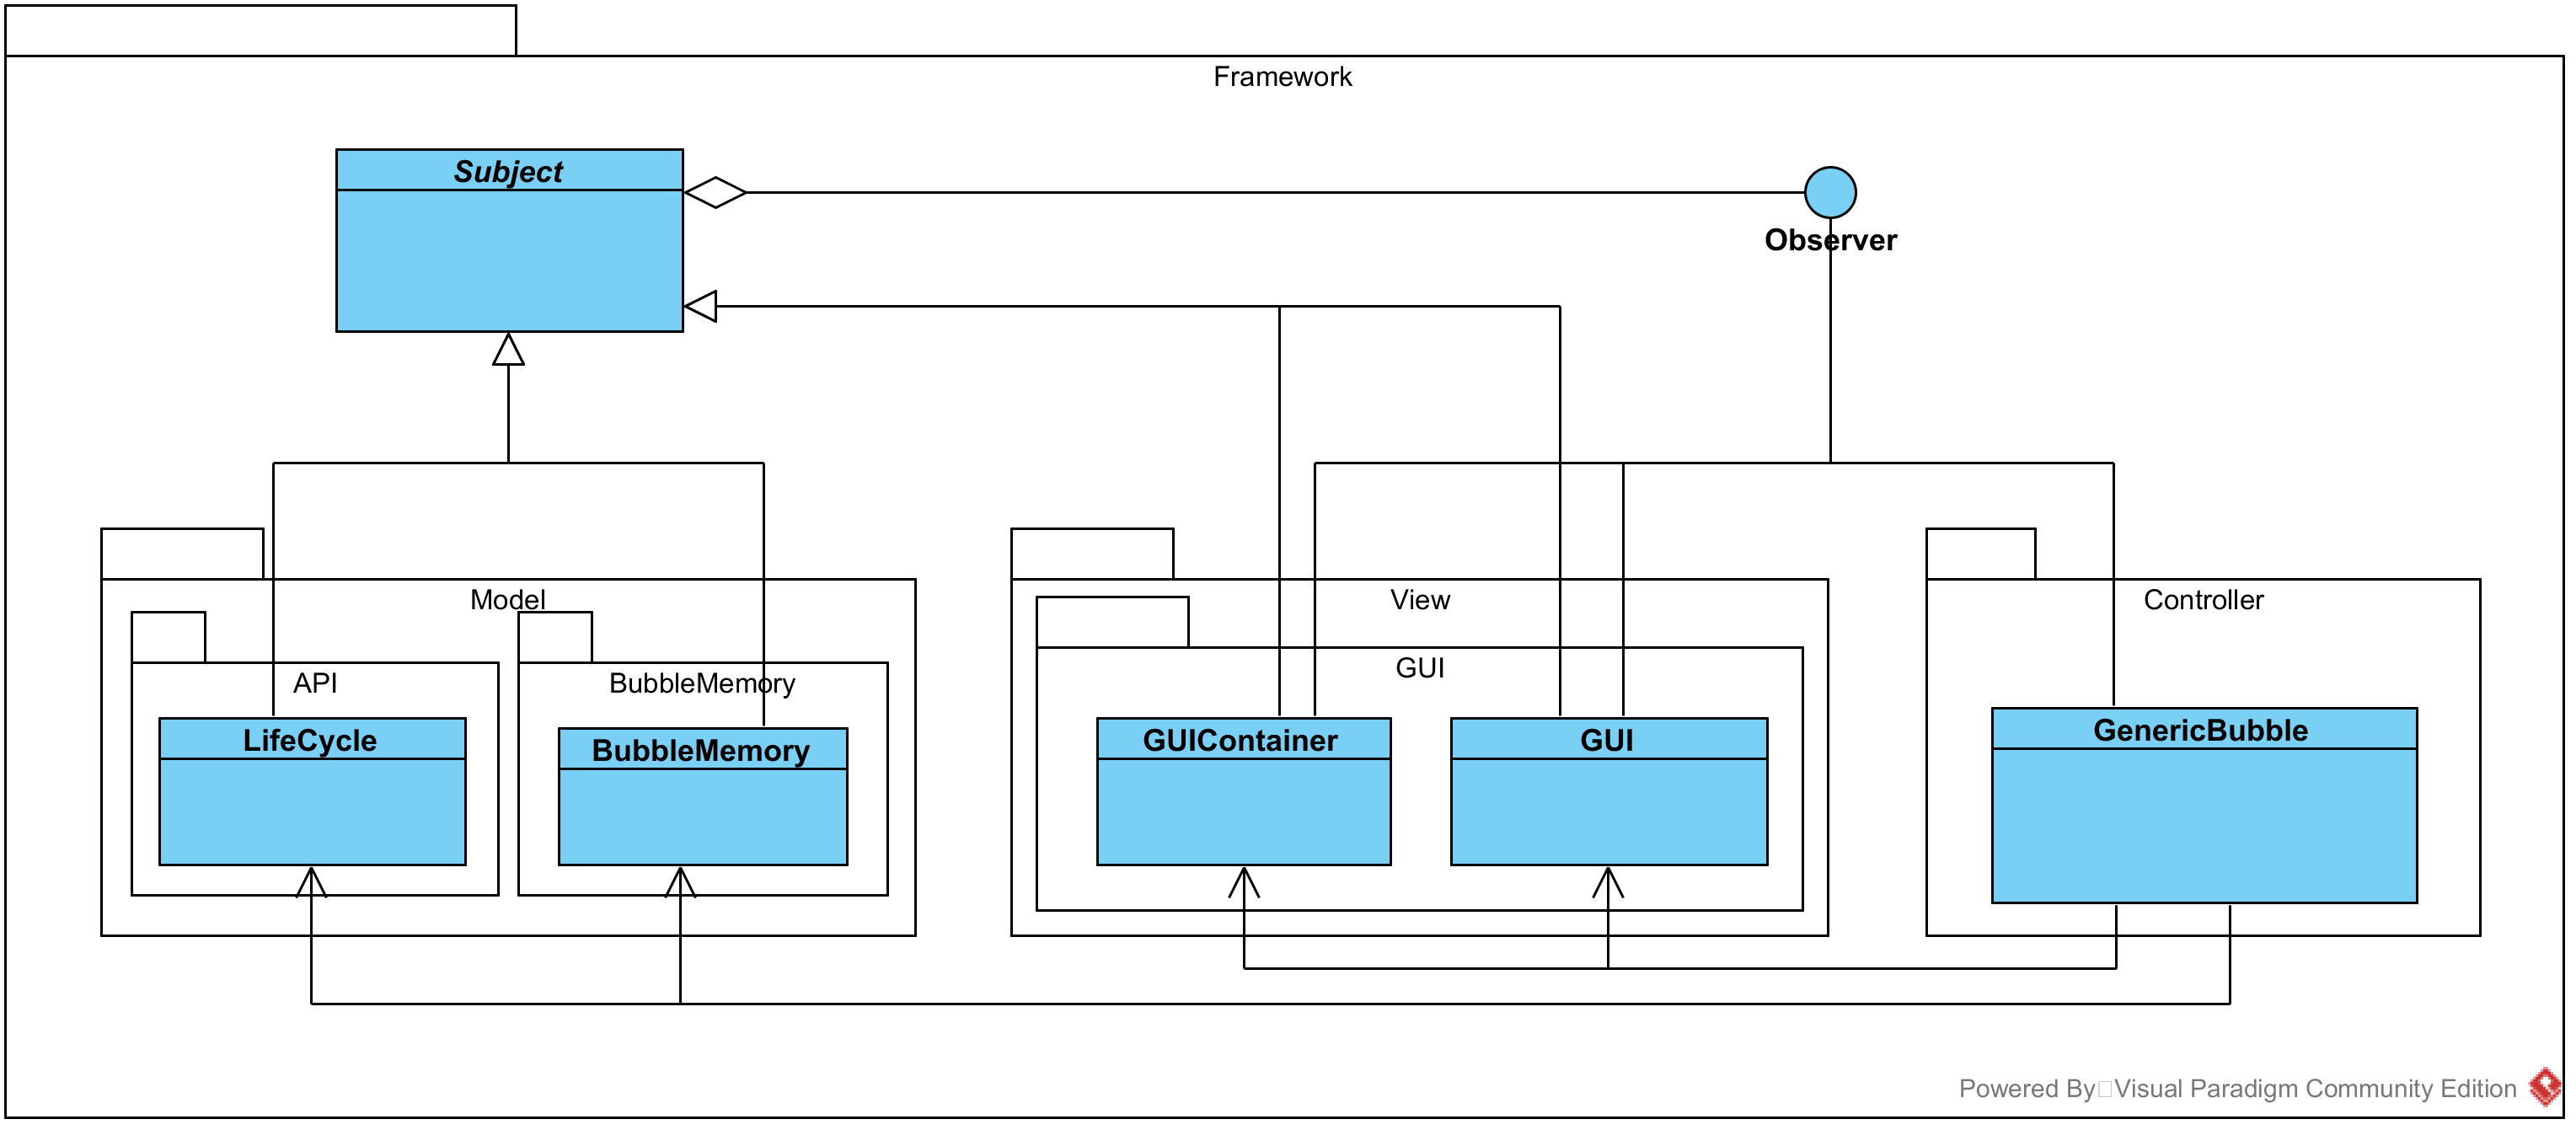
\includegraphics[width=15cm]{./diagrammi_img/applicazione_pattern/mvc_framework.png}
	\caption{Esempio di applicazione pattern MVC all'interno del framework}
\end{figure}

%\subsection{Design Pattern Creazionali}

%\subsubsection{Singleton}
%\textbf{Scopo:} \\
%Permette di vincolare le classi che devono avere una sola istanza durante l'esecuzione dell'applicazione.\\
%\textbf{Utilizzo:} \\
%Viene utilizzato per l'interfaccia che gestisce la comunicazione col database MongoDB e per i controller delle strutture MVC presenti nel framework e nella bubble To-do list. Viene inoltre utilizzato nella classe Order\-Gateway, la quale necessita di rappresentare un'unica istanza per ogni sistema (Ristorante).

\subsection{Design Pattern Strutturali}

%\subsubsection{Fa\c{c}ade}
%\textbf{Scopo:} \\
%Fornisce un'interfaccia unica per un sottosistema più complesso, rendendo visibili solamente alcune parti agli altri oggetti. Rendendo unico il punto d'accesso vengono minimizzate le comunicazioni e le dipendenze. Fa\c{c}ade inoltre non impedisce l'utilizzo delle classi interne al sottosistema, creando un compromesso tra facilità d'uso e generalità. \\
%\textbf{Utilizzo:} \\ 
%Fa\c{c}ade viene utilizzato per creare un livello astratto all'interno della view. Viene infatti delegato alla classe \glossario{GUI} il compito di indirizzare le richieste ricevute dal controller al giusto componente interno. Vengono in questo modo semplificate le comunicazioni, viene ridotto l'accoppiamento e quindi aumentata la portabilità.
%
%\begin{figure}[H]
%	\centering
%	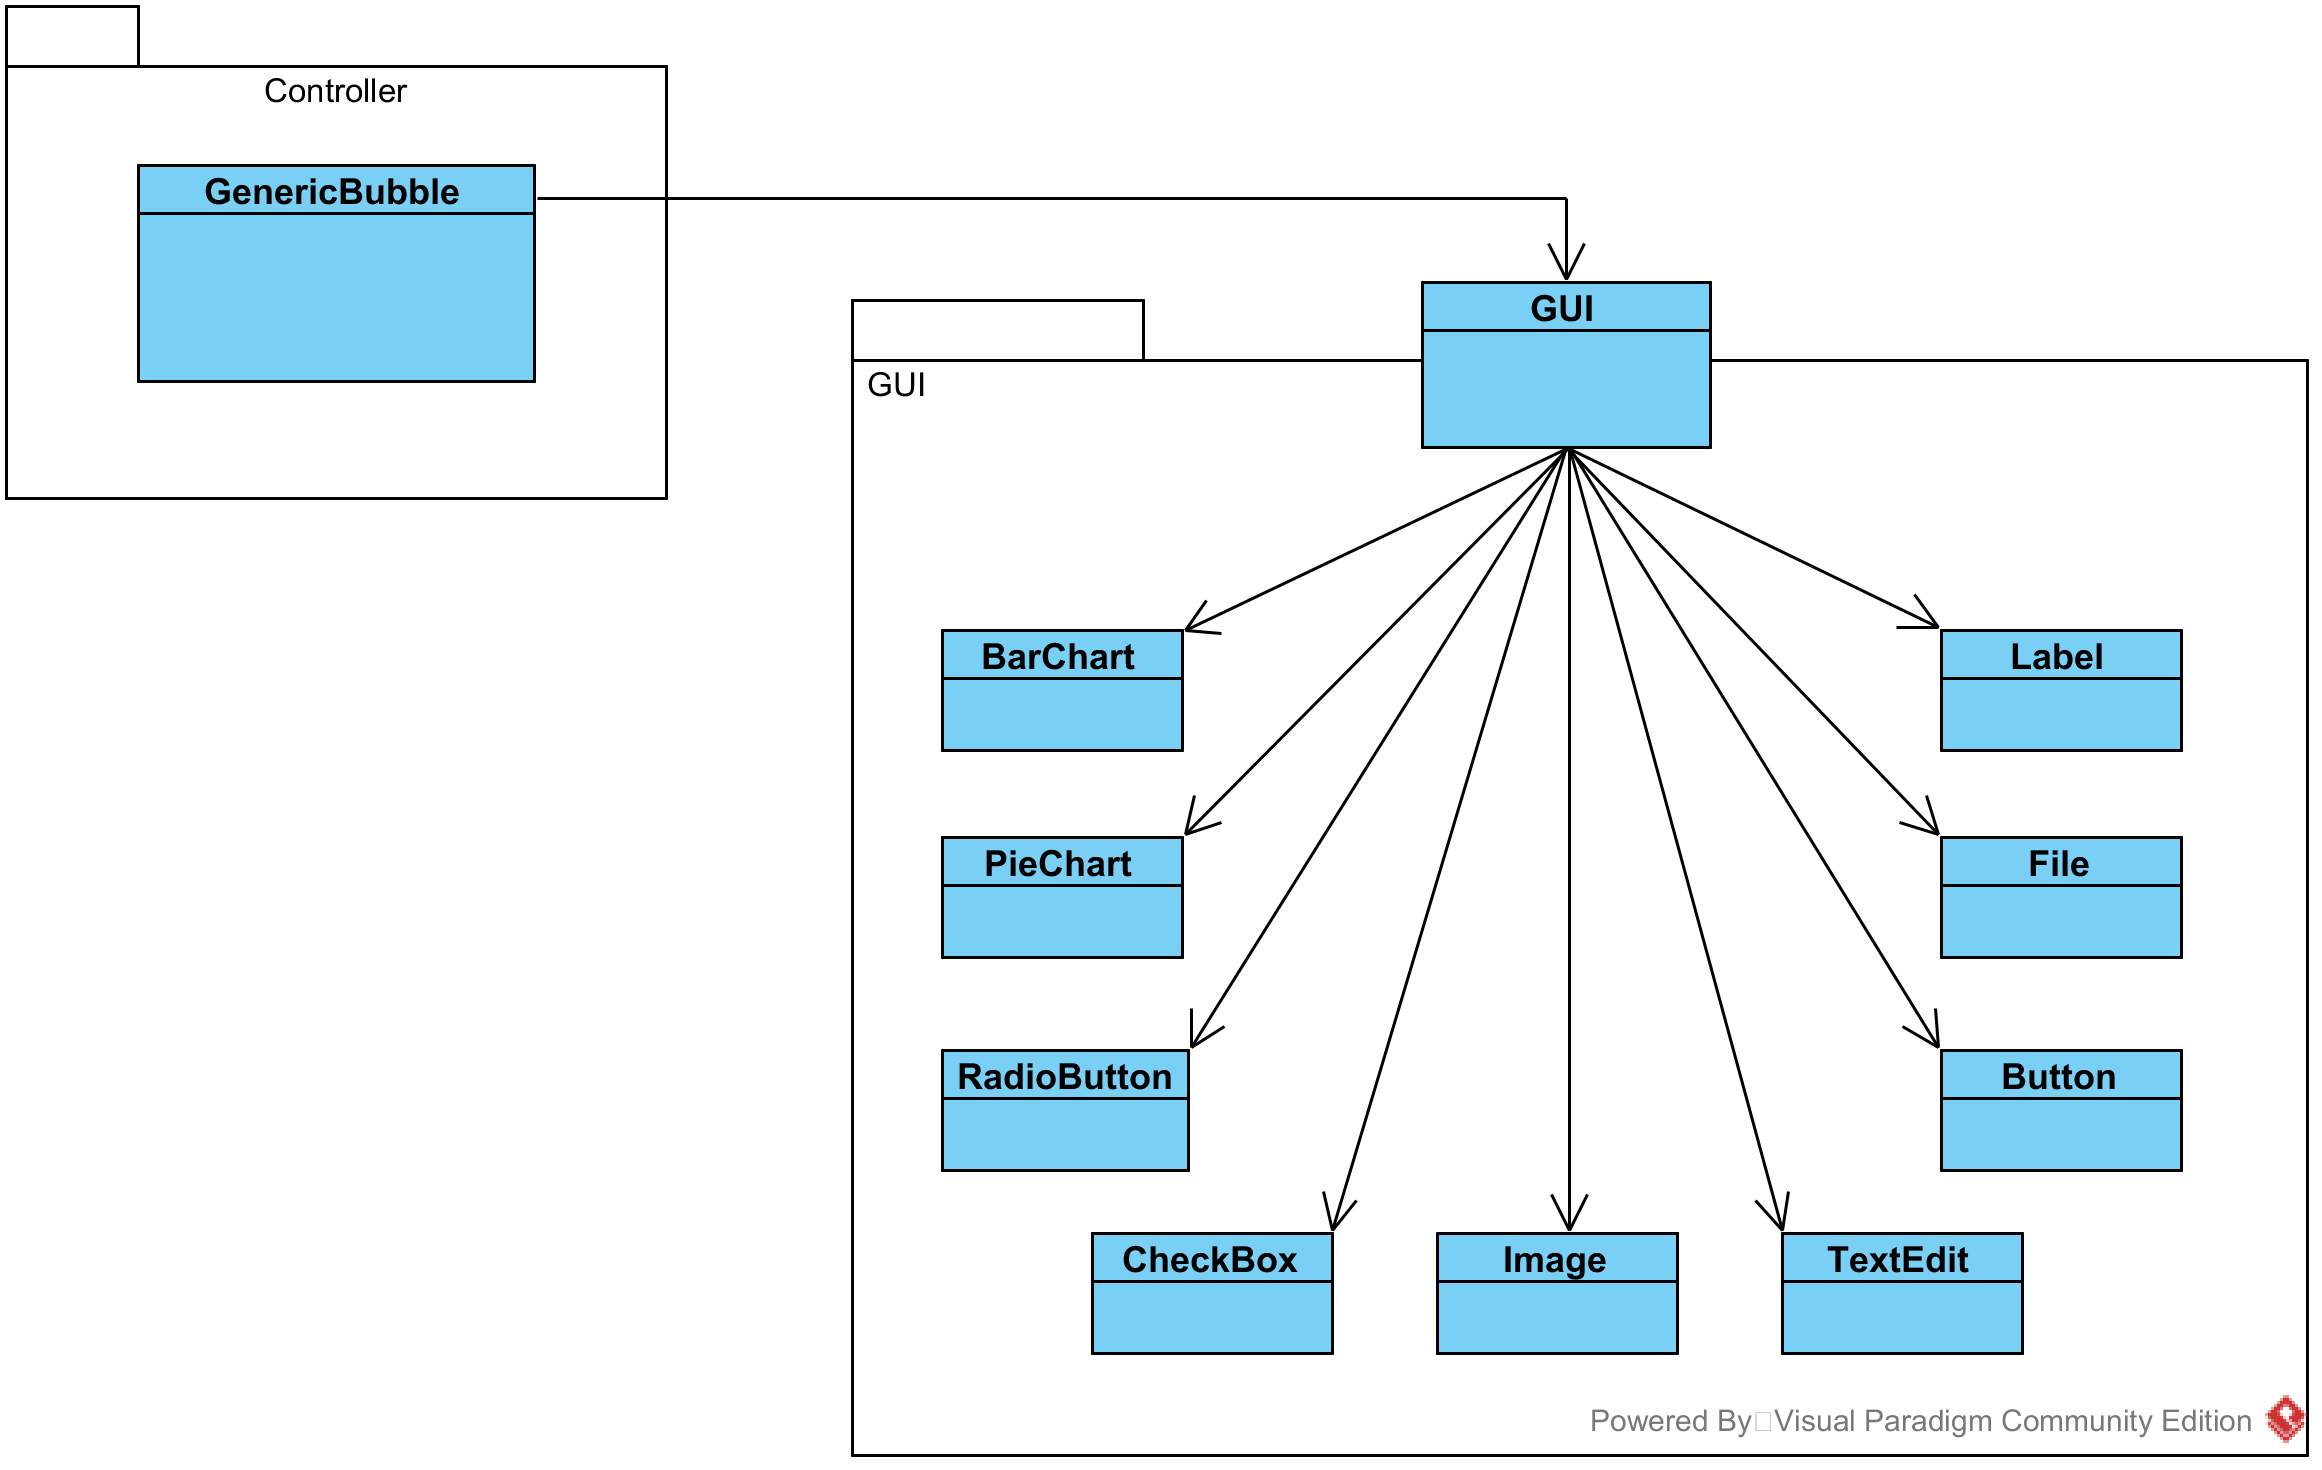
\includegraphics[width=15cm]{./diagrammi_img/applicazione_pattern/facade_framework.png}
%	\caption{Applicazione pattern fa\c{c}ade all'interno del framework}
%\end{figure}

\subsubsection{Proxy}
\textbf{Scopo:}\\
Fornisce un surrogato per un altro oggetto, per controllarne l'accesso.\\
\textbf{Utilizzo:}\\
Questo pattern viene utilizzato per avere una rappresentazione locale degli oggetti remoti, in particolare per le comunicazioni che avvengono tra l'OrderGateway e le varie bubble.

\begin{figure}[H]
	\centering
	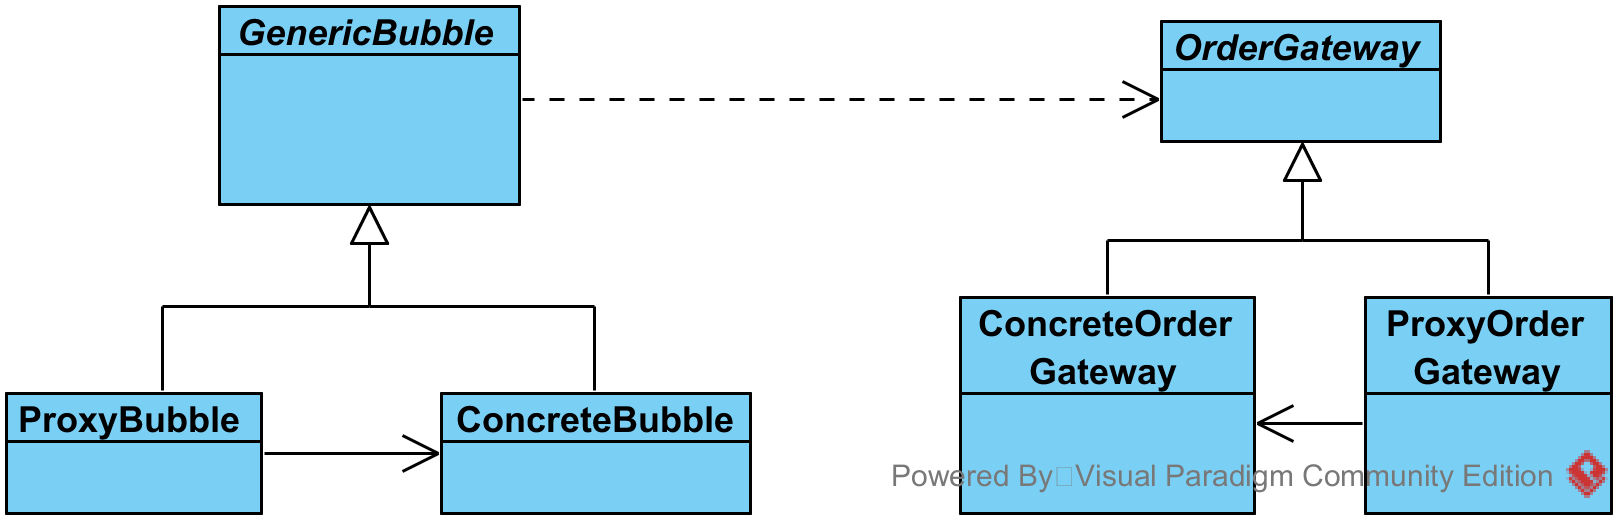
\includegraphics[width=15cm]{./diagrammi_img/applicazione_pattern/proxy_demo.png}
	\caption{Applicazione pattern proxy all'interno della bubble Bubble \& eat}
\end{figure}

\subsubsection{Module}
\textbf{Scopo:} \\
Rende disponibile all'interno degli oggetti l'encapsulation, rendendo \textit{private} e non accessibili dall'esterno campi dati e funzioni utilizzate come campi intermedi.\\
\textbf{Utilizzo:} \\
Verrà utilizzato questo design qualora nella scrittura dell'oggetto debbano esserne rese private alcune parti. In particolare, questo pattern viene associato al pattern fa\c{c}ace.
\begin{figure}[H]
	\centering
	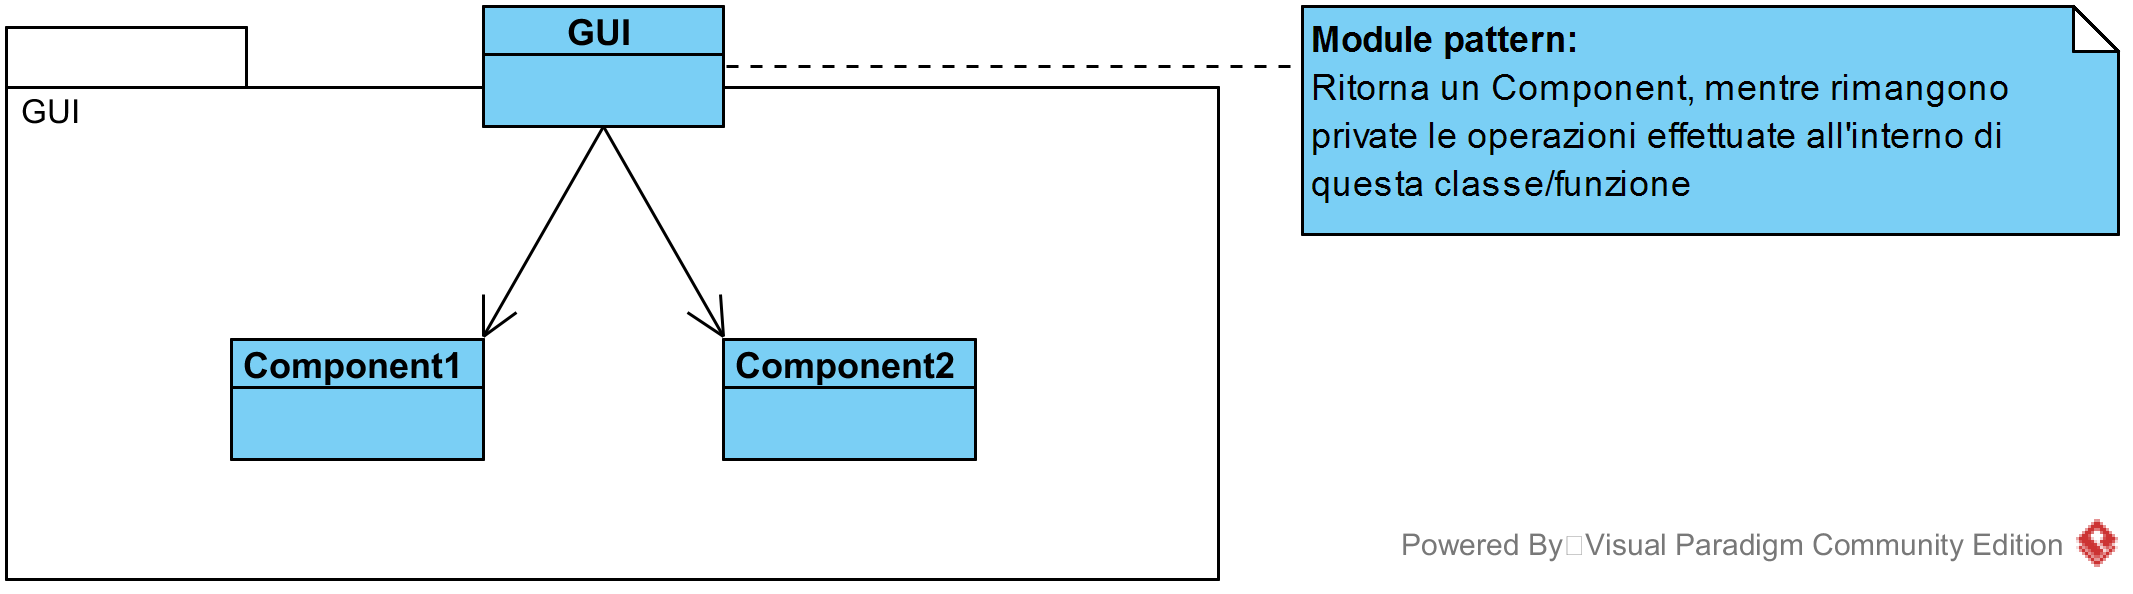
\includegraphics[width=15cm]{./diagrammi_img/applicazione_pattern/module_framework.png}
	\caption{Applicazione pattern module all'interno della bubble Bubble \& eat}
\end{figure}

\subsection{Design Pattern Comportamentali}\label{DesignPatterComportamentali}

\subsubsection{Observer}
\textbf{Scopo:} \\
Permette l'aggiornamento di più viste contemporaneamente, disinteressandosi di quante o quali esse siano.\\
\textbf{Utilizzo:} \\
Verrà usato per sincronizzare le varie bubble che opereranno con dati condivisi, in modo da mantenerle sempre aggiornate e consistenti le une con le altre. Allo stesso modo l'OrderGateway contiene al suo interno un observer per gestire la connessione e la sincronizzazione degli eventi.
\begin{figure}[H]
	\centering
	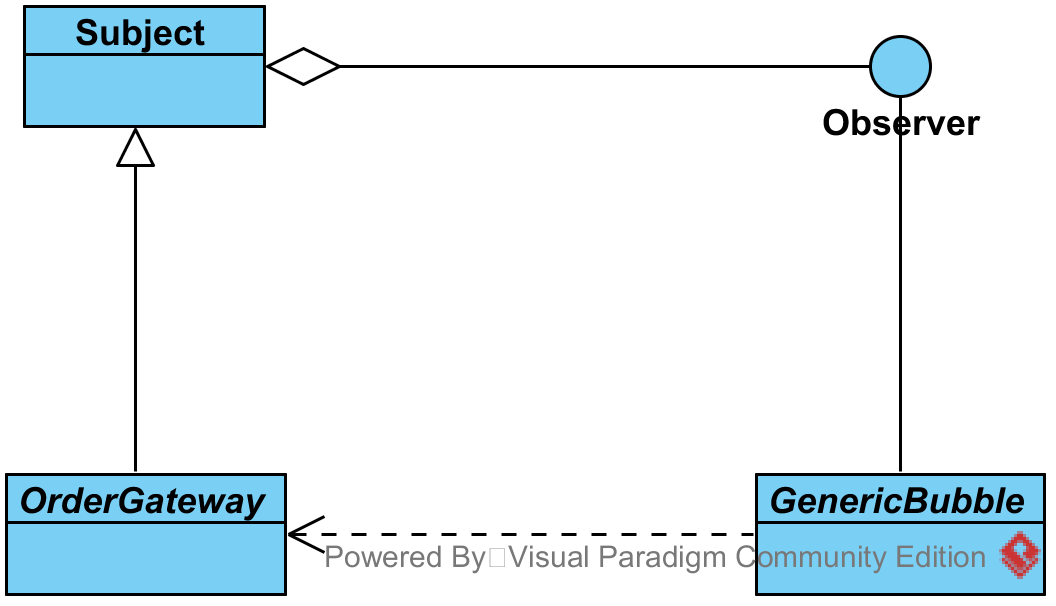
\includegraphics[width=10cm]{./diagrammi_img/applicazione_pattern/observer_demo.png}
	\caption{Applicazione pattern observer all'interno della \DemoName}
\end{figure}

\subsubsection{Strategy}
\textbf{Scopo:} \\
Definisce una famiglia di algoritmi, li incapsula e li rende interscambiabili. Il pattern strategy permette di variare l'algoritmo, indipendentemente dai clients che lo utilizzano.\\
\textbf{Utilizzo:} \\
Questo pattern verrà usato per indirizzare le informazioni dell'OrderGateway alla bubble corretta, tramite un handler interno ad esso.
\begin{figure}[H]
	\centering
	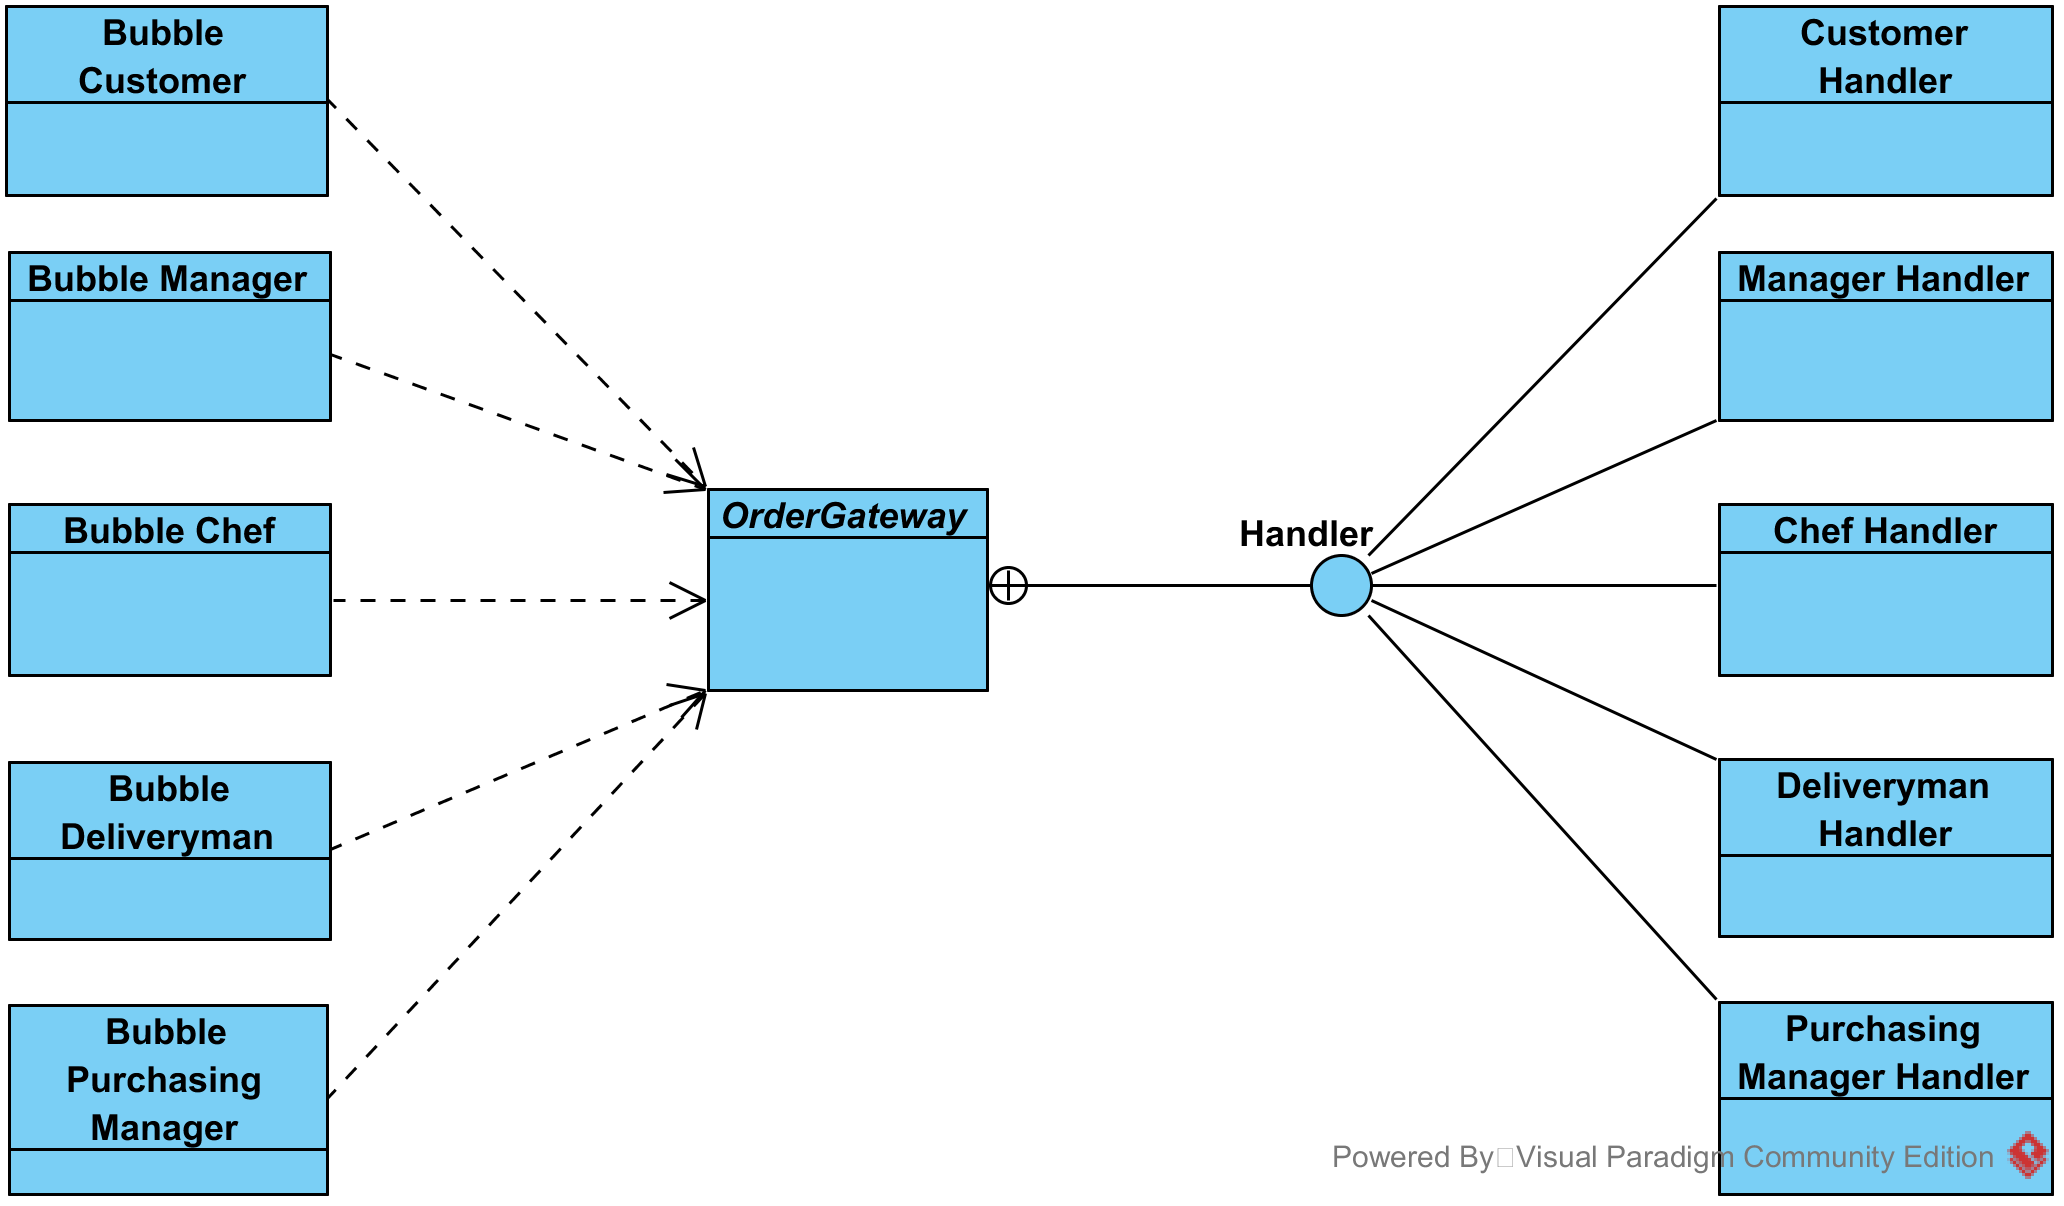
\includegraphics[width=15cm]{./diagrammi_img/applicazione_pattern/strategy_demo.png}
	\caption{Applicazione pattern strategy all'interno della \DemoName}
\end{figure}